\documentclass{article}
\usepackage[utf8]{inputenc}
\usepackage[portuguese]{babel}
\usepackage{float}
\usepackage{hyperref}

\hypersetup{
    colorlinks=true,
    linkcolor=black,
    filecolor=blue,      
    urlcolor=blue,
    citecolor=black,
}

\title{Modelagem da Pandemia do COVID-19 na Suécia}
\author{João Pedro de Abreu Marciano }
\date{}

\usepackage{natbib}
\usepackage{graphicx}

\begin{document}

\maketitle

\section{Introdução}
Desde o ínicio da pandemia, países têm tomado diferentes medidas para diminuir a transmissão da doença enquanto não há vacinas ou tratamentos altamente efetivos. Isso é necessário pelos altos índices de hospitalização e mortos da doença.

A Suécia foi um dos países que divergiu da maioria dos outros países da Europa na estratégia de mitigação da pandemia. O país decidiu não fazer o lockdown, utilizou poucas medidas mandatórias e priorizou incitar a responsabilidade individual na população. Há alguns estudos que comparam como essa abordagem se saiu em comparação com a de outros países. 

No geral, ela não foi boa como demonstrado em \citep{managing}. E, além disso, o artigo \citep{pandemicshutdown} apresenta como não ouve diferenças extremamente significativas na movimentação econômica do país em relação a seus países vizinhos.

Apesar disso, a chamada de segunda onda do vírus, que tem ocorrido em grande parte dos países europeus, não está ocorrendo na Suécia atualmente. O país possui uma das menores médias de infectados diários per capita do continente europeu.

A situação atual do país é de leve crescimento no número de infectados e menos de 5 mortes diárias.

Há alguns artigos que modelaram a transmissão doença na Suécia. Abaixo segue um pequeno resumo de alguns deles.

Em \citep{managing}, o principal objetivo do trabalho é modelar como outras medidas de mitigação se sairiam em comparação com outras medidas que poderiam ser tomadas.

O gráfico abaixo presente no artigo é um dos resultados.

\begin{figure}[H]
    \centering
    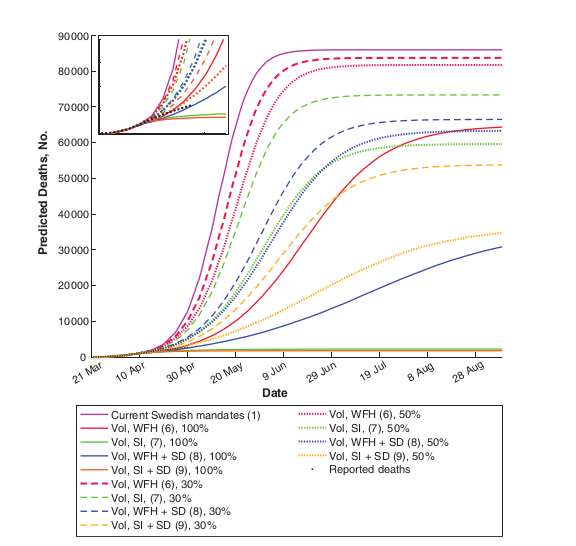
\includegraphics[scale=0.6]{corona.png}
    \caption{Predicted  coronavirus  disease  2019  (COVID-19)  deaths  in  Swedenwith different voluntary adherence strategies.  Plotted are median numbers ofCOVID-19 deaths predicted by modeling current Swedish public health manda-tes and individual voluntary behaviors.  These are compared against reportedCOVID-19 deaths in Sweden.  A mod- erate level of individual self-isolation (SI)is sufficient to well reproduce the reported death tolls.  Data are shown for 3-daydoubling times (see Supplementary Figures 4 and 5 for alternates).  Numbers inparentheses represent interventions listed in Methods.  April predictions are en-larged in the inset.  Abbreviation:  SD, social distancing; Vol, Voluntary; WFH,work from home.  Fonte: \citep{managing}.}
    \label{fig:my_label}
\end{figure}

Outro trabalho é \citep{modelstudies} em que são utilizados os modelos SI e SIR para modelar o início da pandemia no país, já que o artigo é de 6 de abril de 2020. Os resultados foram bem satisfatórios para os dados disponíveis na época.

Os dois trabalhos que são a principal inspiração para este são os \citep{thefirst100days} e \citep{multiwave} dos mesmos autores. No primeiro artigo eles introduzem o modelo forced-SIR (FSIR) que será mais detalhado na seção \ref{Metodologia}, e com ele modelam de maneira bem satisfatória os primeiros 100 dias da pandemia. No segundo artigo, os autores percebem que as diferentes intervenções governamentais e as disseminações centralizadas em diferentes centros urbanos geram um comportamento de múltiplas ondas epidêmicas nos dados, chamadas de subepidemias (veja \ref{fig:my_label2}). Dado isso, eles estendem o modelo FSIR para um modelo de multiplas ondas. Este será o modelo utilizado neste artigo e será mais aprofundado na seção \ref{Metodologia}.

\begin{figure}[H]
    \centering
    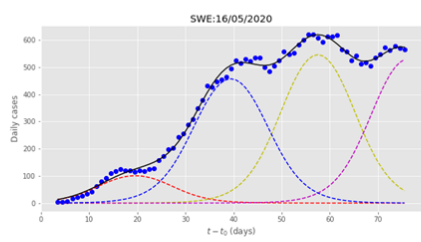
\includegraphics[width=0.8\linewidth]{corona2.png}
    \caption{Subepidemias na Suécia. Fonte: \citep{multiwave}}
    \label{fig:my_label2}
\end{figure}

\section{Metodologia}
\label{Metodologia}
Primeiro será necessário apresentar o modelo forced-SIR (FSIR) introduzido em \citep{thefirst100days}. Este modelo é uma adaptação do modelo SIR. Na verdade, a transmissão do coronavirus se assemelha aos compartimentos do modelo SEIR, mas, por simplicidade, vamos considerar I do modelo SIR como um acoplamentos dos compartimentos E e I do modelo SEIR. Vamos considerar também uma população fixa $N$. Temos então os seguintes compartimentos

\begin{itemize}
    \item 
    $S(t)$ indivíduos suscetíveis a doença;
    \item
    $I(t)$ indivíduos infectados ou infecciosos;
    \item
    $R(t)$ indivíduos removidos do grupo de infectados, seja adquirindo imunidade ou falecendo.
\end{itemize}

E o modelo SIR possui dois parâmetros $\beta, \gamma > 0$:

\begin{itemize}
    \item $\beta$ descreve a taxa efetiva de contato da doença. Um indivíduo infectado entra em contato com $\beta$ outros indivíduos por unidade de tempo;
    
    \item $\gamma$ é a taxa média de remoção, ou seja, $\frac{1}{\gamma}$ é o período médio de tempo durante o qual um indivíduo infectado pode transmitir a doença antes de ser removido.
\end{itemize}

O comportamento do modelo SIR e descrito pelas equanções diferenciais:

$$\frac{dS}{dt} = -\beta I \frac{S}{N}$$

$$\frac{dI}{dt} = \beta I \frac{S}{N} - \gamma I$$

$$\frac{dR}{dt} = \gamma I$$

Muito trabalhos tem tentado fazer os parâmetros como função do tempo para modelar a pandemia. O \citep{thefirst100days} é um deles. Colocando um decaimento exponencial em $\beta$, baseado nas soluções numéricas, os autores estimaram como seriam as soluções de forma bem simples. $\beta$ com decaimento exponencial modela muito bem o chamado de "achatamento" da curva. Assim, chegaram no seguinte resultado:

$$\tilde{S} = N-\frac{N'}{1+e^{-\alpha_1(t-t_1)}}$$
$$\tilde{R} = \frac{N'}{1+e^{-\alpha_2(t-t_2)}}$$
$$\tilde{I} = \frac{N'}{1+e^{-\alpha_1(t-t_1)}}-\frac{N'}{1+e^{-\alpha_2(t-t_2)}}$$

onde $N',\alpha_1,\alpha_2,t_1,t_2$ são tratados como parâmetros ajustáveis, com $t_1$ e $t_2$ sendo os tempos em que as populações $\tilde{S}$ e $\tilde{R}$ atingem o ponto médio dos sigmóides, respectivamente. A taxa de diminuição da população suscetível é capturada pelo valor de $\alpha_1$ e a taxa de aumento da população removida é capturada pelo valor de $\alpha_2$.

Este é um modelo simples é de extrema eficácia. O modelo que será utilizado neste trabalho é o Multiple Wave Forced-SIR introduzido em \citep{multiwave}. Nesse modelo, decidiremos manualmente quantas curvas do modelo FSIR se adequam aos dados. Após isso, um método de otimização será utilizado para cada um dos parâmetros de cada uma das curvas de forma que a soma delas represente o comportamento apresentado nos dados.

Optamos por utilizar este modelo no trabalho, pois sua adequação aos dados se mostrou fácil e efetiva. Além disso, como as intervenções governamentais na Suécia foram diferentes das adotadas no restante do mundo, modelá-las seria mais complicado. Esse modelo consegue simular de maneira satisfatória, apenas baseado nos dados, essas intervenções, já que isso é capturado pelas múltiplas ondas.

Para a proxima seção, os dados serão retirados do csv disponibilizado pelo \href{https://ourworldindata.org/coronavirus}{Our World in Data} (\citep{ourworldindata})

\section{Resultados}

\section{Discussão e Conclusão}

\nocite{*}

\bibliographystyle{plain}
\bibliography{references}
\end{document}
